\section{Neural Networks}\label{sec:NN}
The concept of a \ac{NN} has been around for more than 80 years, and today they are one 
of the most popular and successful \ac{ML} methods. The key to its popularity stems from
its versatility, achieving high performance in a large range of both regression 
and classification problems. One of the defining qualities in a \ac{NN} is the 
possibility of diverse architecture, meaning that there are many
categories of \ac{NN}, where each category has an even deeper selection of
networks. Categories ranging from \ac{CNN}, \ac{RNN} to simple \ac{FFNN}, where each
category is specified for their own set of problems. In this section I will introduce 
some fundamental definitions in regard to \ac{NN}, and go through the underlying 
algorithm of the back- and forward propagation.

\subsection{General Structure}
There are often drawn comparisons between the structure of the neural network, 
and the way the human mind operates, hence neural. Similarly to the human mind, a \ac{NN} is 
composed of different neurons, or nodes communicating information backwards and forwards in different 
regions. In the case of a neural network we call these regions layers. All layers
are composed of a specified number of nodes. A \ac{NN} has three types of layers;
\emph{input layer}, \emph{hidden layer} and \emph{output layer}. There is only one input layer, and it has
the same number of nodes equal to the number of features for each data point. 
There can be an arbitrary number of hidden layers, with each hidden layer containing
an arbitrary number of nodes. Finally, the \ac{NN} has an output layer. The output layer
contains a number of nodes equal to the dimensions of the target.
\\
A \ac{NN} functions by passing information in between the different layers through 
nodes. The nodes are simply pockets of information, each containing a value. 
All the nodes in the input layer are (in most cases) connected to all nodes in the nearest hidden layer,
and likewise said hidden layer is connected to the next hidden layer. This structure continues
until we reach the final layer, the output layer. The structure is illustrated in figure
\ref{fig:NN}. The figure shows a simple \ac{NN} with a two-dimensional data set (two nodes in input layer),
two hidden layers with three nodes each and a one-dimensional target value. It also illustrates 
how a \ac{NN} aims to map from data to a prediction.
\begin{figure}
    \centering
    \vspace*{-12.5mm} 
    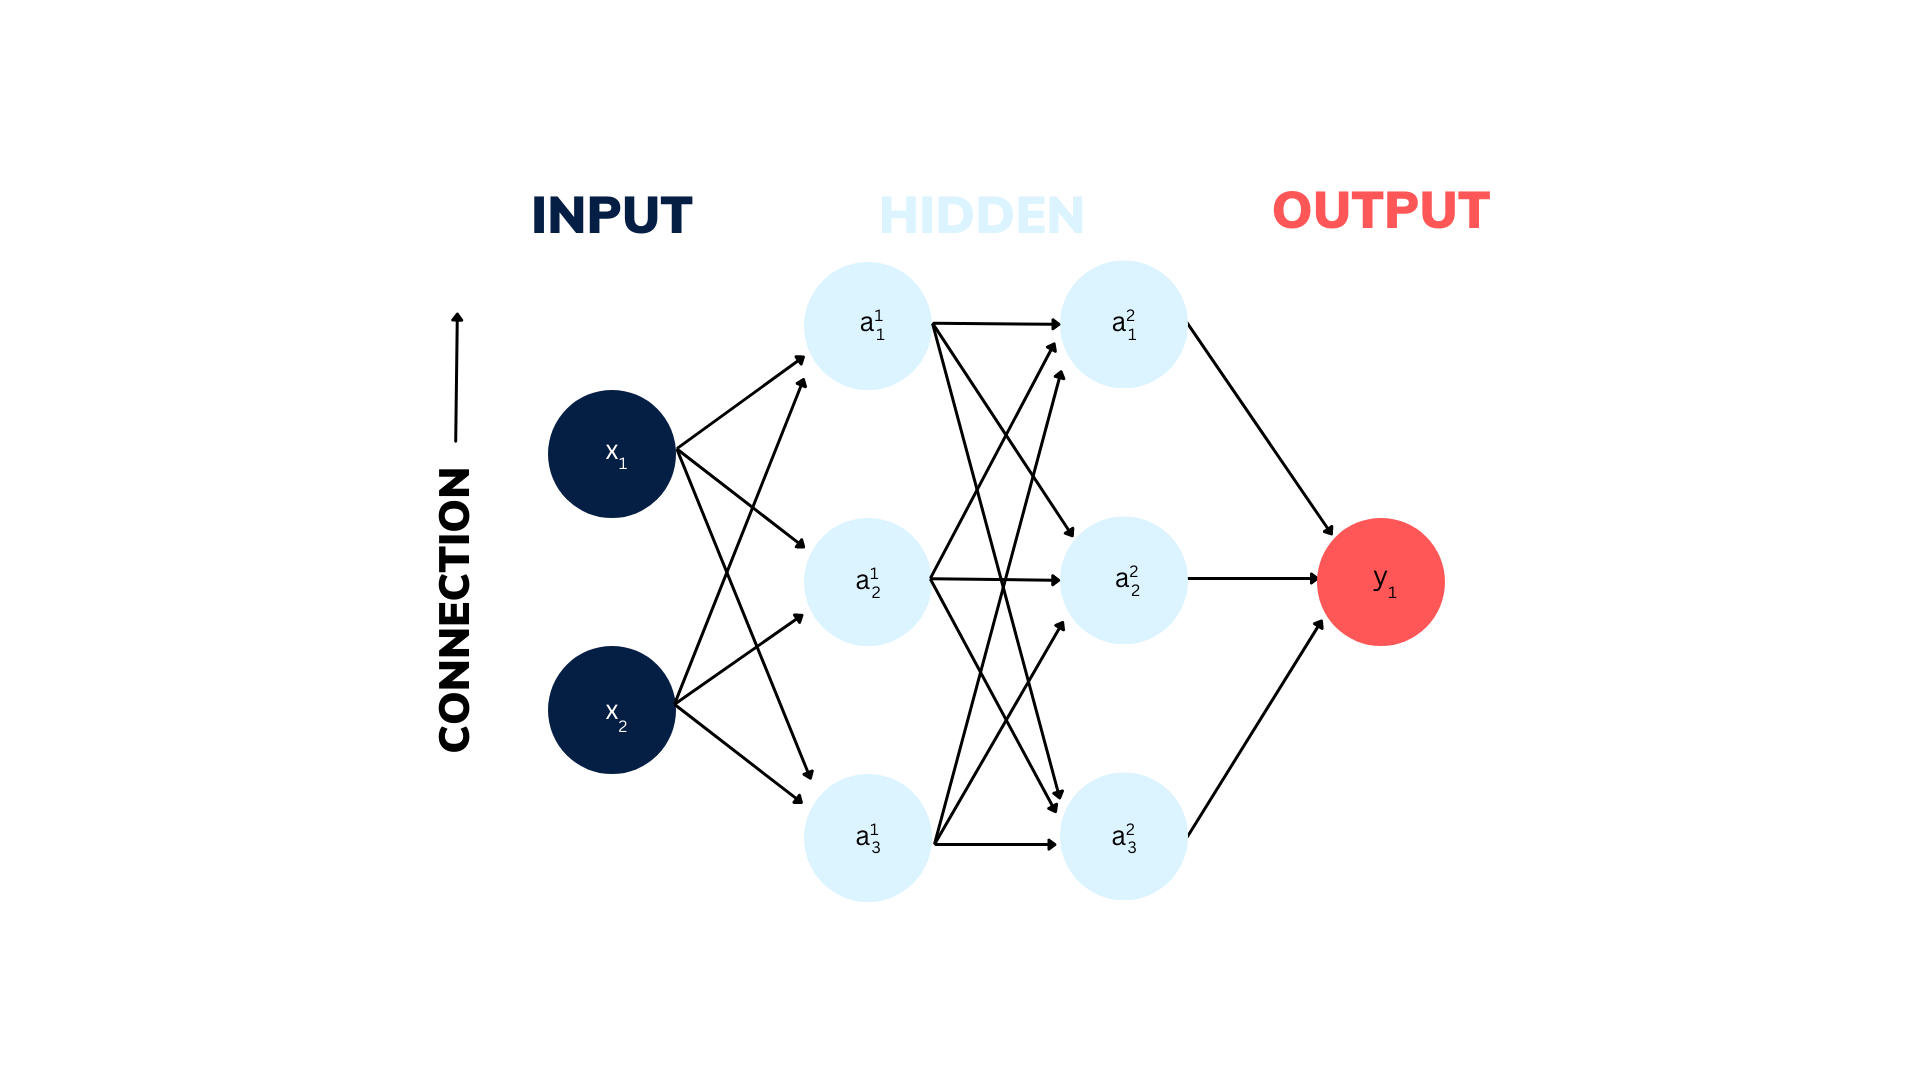
\includegraphics[width=0.9\textwidth]{Figures/Illustrations/Input_labels.png}
    \vspace*{-12.5mm} 
    \caption{An illustration of the architecture of a \acs{NN} with two hidden layers.}
    \label{fig:NN}
\end{figure}
In figure \ref{fig:NN} we can see how all the different nodes are connected, illustrated by 
the arrows. The passing of values between different nodes are controlled by a set of weights and
bias parameters. These parameters are defined for each connection and are what will be tuned 
during training. The weights and biases for a given connection of two nodes, defines the effect one node 
has on the other.
\\
In a traditional \ac{FFNN} the information is passed linearly (in figure \ref{fig:NN}, from left to right) 
in a process we call \emph{forward propagation}. Other variants can include the information taking a more 
complex route. It is often the route from input- to output layer that categorizes the type of \ac{NN}. In 
this report I used a set of simple \ac{FFNN}'s. 

\subsection{Feeding Forward}\label{subsec:FP}
With the structure described in the previous section, a trained model, $\mathcal{F}$, produces a prediction,
$Y$, for a data set, $X$, by passing information from input layer, through all hidden layers, to the output layer, 
which we call forward-propagation. In this section I aim to explain the underlying algorithm and math used by the 
\ac{NN} to map input to output. 
\\
We imagine the passing from hidden layer $l-1$ to $l$, where $l \in \{2,...,L \}$\footnote{There is a special
case for when $l=1$ which will be addressed in the next paragraphs.} and $L$ is equal to the
number of hidden layers. The activated value of a node in layer $l$, is defined as $a^l_j$ (as indicated by figure \ref{fig:NN}), 
where $j\in \{0,1,...,N_l\}$ and $N_l$ is equal to the number of nodes in $l$. The value of $a_j^l$ is defined as 
the \emph{activated} sum of all nodes in the previous layer, $a_j^{l-1}$ where the sum is weighted by a parameter $\bf{w} \sf _j^l$ 
and shifted by the bias, $b^l_j$ for $j\in \{0,1,..., N_{l-1} \}$. The activated value of a node j in layer l is defined as 
\begin{align}\label{eq:activated}
    z_j^l = \sum_{k=1} ^ {N_{l-1}} w_{kj}^la_k^{l-1} + b^l_j,
\end{align}
where $w_{kj}^l$ corresponds to the weight in $\bf{w} \sf _k^l$ specific for the connection between node k and j.
\\
To attain the full activated value, $a_j^l$ we pass $z_j^l$ through the \emph{activation function}. The activation function, $\sigma^l$ 
is a generally non-linear function used to control the limit or expand the value range for the node values. The activation 
function is general for all nodes in a given layer, but can vary in between layers. Therefore,
we find $a_j^l$ by the equation
\begin{align}\label{eq:ajl}
    a_j^l = \sigma \left (\sum_{k=1} ^ {N_{l-1}} w_{kj}^la_k^{l-1} + b^l_j\right ) = \sigma^l(z_j^l).
\end{align}
A more detailed illustration of the information passed from one layer to a node in the next layer is displayed 
in figure \ref{fig:WB}. In figure \ref{fig:WB}, we see all steps described in the process; \emph{(1)} all nodes in 
l-1 are summed with a corresponding weight, \emph{(2)} the sum is shifted by a constant term (bias), \emph{(3)} the 
scaled and weighted sum defines the inactivated value $z_j^l$, \emph{(4)} we define $a^l_j$ by passing the 
sum through $\sigma^l$.  
\begin{figure}
    \centering
    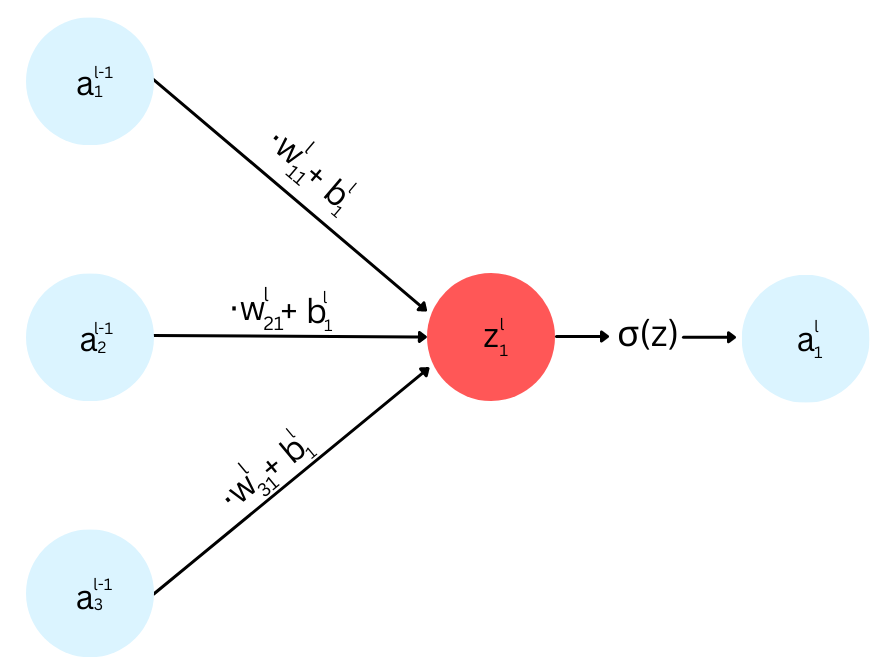
\includegraphics[width=0.5\textwidth]{Figures/Illustrations/WeightBias.png}
    \caption{An illustration of a forward propagation from one layer to a node in the next.}
    \label{fig:WB}
\end{figure}
This method is used to pass information between all layers, except between the first and the second. 
In this case we simply replace the activated term, $a_k^{l-1}$ in equation \ref{eq:ajl}, by the input data,
$x_i$ for $i\in\{0,1,...,N\}$, where N is equal to the number of features for the data. In the case $l=1$, \ref{eq:ajl} 
becomes
\begin{align}
    a_j^1 = \sigma \left (\sum_{k=1} ^ {N} w_{kj}^1x_k + b^1_j\right ) = \sigma(z_j^1).
\end{align}
And in the case where $l=L$, $a_j^L$ is equal to the final output. 
\subsection{Back Propagation}\label{subsec:BP}
The backward propagation acts as the engine that drives the training of a neural network. It has the purpose
of calculating the gradients of the \emph{cost function}, $\mathcal{C}$, with respect to the weights and biases of the network. 
The cost function defines to which metric we aim to optimize the network. When a neural network produces a prediction, $Y$, the error in the prediction
is defined by the cost function as $\mathcal{C}\left(Y, T\right)$, where T is the target. To minimize $\mathcal{C}$, the 
backward propagation utilizes the gradient with respect to the weights and biases in the network, as described in the section 
regarding optimization \ref{sec:Opti}. Instead of a direct calculation of the gradient, which is very computationally heavy, 
the backward propagation aims to calculate the gradient through a recursive algorithm which traces the error backwards through 
the network. It is this algorithm I will describe in this section.
\\
When minimizing the error defined by $\mathcal{C}$, we can apply several optimization algorithms described in 
section \ref{sec:Opti}. Common for the algorithms is the use of the gradient of the cost function with regard to 
the tunable parameters. In our case these parameters are the weights and biases, $w_{i,j}^l$ and $b^l_j$. The goal of 
the backward propagation is therefore to calculate the gradients $\partial \mathcal{C}/\partial w_{i,j}^l$ and
$\partial \mathcal{C}/\partial b^l_j$. 
\\
To begin with we can derive an expression for $\partial \mathcal{C}/\partial w_{i,j}^l$. We use the chain-rule to define 
\begin{align*}
    \frac{\partial \mathcal{C}}{\partial w_{i,j}^l} = \frac{\partial \mathcal{C}}{\partial z^l_j} \frac{\partial z^l_j}{\partial w_{i,j}^l},
\end{align*}
which we can simplify further by using equation \ref{eq:activated} to calculate the second term, which becomes
\begin{align*}
    \frac{\partial \mathcal{C}}{\partial w_{i,j}^l} = \frac{\partial \mathcal{C}}{\partial z^l_j} a^{l-1}_i.
\end{align*}
We can redefine the first term in the equation above as $\delta_j^l$ and write
\begin{align*}
    \delta_j^l \equiv \frac{\partial \mathcal{C}}{\partial z^l_j}
               = \sum_k \frac{\partial \mathcal{C}}{\partial z^{l+1}_k}\frac{\partial z_k^{l+1}}{\partial z^l_j}  
               = \sum_k \delta_k^{l+1}\frac{\partial z_k^{l+1}}{\partial z^l_j},
\end{align*}
where we have again used the chain rule for all contributing nodes. To calculate the final partial derivative we write
\begin{align*}
    \frac{\partial z_k^{l+1}}{\partial z^l_j} = \frac{\partial z_k^{l+1}}{\partial a^l_j}\frac{\partial a^l_j}{\partial z^l_j}
                                              = w_{jk}^{l+1}(\sigma^l(z_j^l))',
\end{align*}
where we have again used equation \ref{eq:activated}. This gives the expression for $\delta_j^l$
\begin{align}\label{eq:delta}
    \delta_j^l  = \sum_k \delta_k^{l+1}w_{jk}^{l+1}(\sigma^l(z_j^l))'  
\end{align}
Finally this gives us the expression
\begin{align}\label{eq:dw}
    \frac{\partial \mathcal{C}}{\partial w_{i,j}^l} = \delta_j^{l} a_j^{l-1}.
\end{align}
Next we want to derive $\partial \mathcal{C}/\partial b^l_k$. We simply use the chain rule and derive
\begin{align*}
    \frac{\partial \mathcal{C}}{\partial b^l_j} = \frac{\partial \mathcal{C}}{\partial z^l_j}\frac{\partial z_j^l}{\partial b^l_j},
\end{align*}
which from equations \ref{eq:delta} and \ref{eq:dw} is simply
\begin{align}\label{eq:db}
    \frac{\partial \mathcal{C}}{\partial b^l_j} = \delta_k^{l} \cdot 1 = \delta_j^{l},
\end{align}
From all three derived expressions, equations \ref{eq:delta}, \ref{eq:dw} and \ref{eq:db} we see that 
to calculate for all $l\in\{0,1,..,N_l\}$ we must first calculate $\delta_j^L$ and apply a recursive propagation.
To calculate $\delta_j^L = \partial \mathcal{C}/\partial z^L_j$ we again apply the chain rule with the assumption of the activated 
node in the cost-function, and we find
\begin{align}\label{eq:deltaL}
    \delta_j^L = \frac{\partial \mathcal{C}}{\partial a^L_j}\left(\sigma^L(z_j^L)\right)'.
\end{align}
This expression, similarly to equation \ref{eq:delta}, is dependent on the choice of $\mathcal{C}$ and 
the activation functions. Now that equation \ref{eq:deltaL} is defined, we can see that the
gradient of the parameters in all other layers can be calculated. A full \emph{epoch} is defined as 
a forward propagation which creates a prediction, followed by a backward propagation which tunes the parameters 
in an attempt to correct the errors in the prediction.
\subsection{Activation Functions}\label{subsec:activation}
As mentioned in previous sections, activation functions define how the weighted sum of the nodes in the previous layer 
define the value of the node in the current. There are many types of activation functions, 
where all have advantages and disadvantages. The choice of activation function for each layer is defined
before training, making it a hyperparameter. The activation functions applied and tested in this thesis are the following:
\begin{center}
\begin{itemize}
    \item  \emph{Sigmoid}\\  
    \begin{align*}
         \sigma{(z)} = \frac{1}{1+e^{-z}} = a \in [0,1]
    \end{align*}
    \item \emph{LeakyReLU}
    \begin{align*}
        \sigma{(z)} = \left(
        \begin{cases}
            z,& \text{if } z\geq 0\\
            \alpha z,              & \text{otherwise}
        \end{cases}\right)
        = a \in (-\infty, \infty),
   \end{align*}
   where $\alpha$ is scalar.
\end{itemize},
\end{center}
where $z$ is an inactivated node which is activated to define $a$, the activation.

\subsection{Network Ensembles, Dropout and LWTA Networks}\label{subsec:LWTA}
So far in the thesis, I have only covered dense layers, meaning that every node in a layer 
is connected to the nodes in the previous and following layer. 
This definition covers many, but not all hidden layers. Some layers do not pass values back and forth between 
nodes but instead dynamically change the architecture of the \ac{NN}. In this analysis, 
I have implemented both the \emph{dropout}-layer, and also a group of layers fitting the definition 
introduced in the paper \cite{srivastava_compete_2013}, as \ac{LWTA}.
\subsubsection*{Dropout}\label{subsubsec:Dropout}
The dropout layer functions by assigning a predetermined probability to each neuron in a given layer. Based on the 
probability, a number of neurons (dependent on the probability) is dropped in each forward pass. By doing this the 
dropout layer creates a different architecture for the network for every round of training. Each unique architecture represents 
its own network in what becomes an ensemble of networks. 
\\
As mentioned in previous sections, creating ensembles of models is a form of regularization. In the case of 
dropout, it minimizes the risk of overfitting by hindering a phenomenon known as complex co-adaptation. Complex
co-adaptation happens when a neuron becomes overly dominant such that neighboring neurons no longer contribute (relative
to the dominant neuron) and therefore lack the motivation to tune. When this happens, networks become fragile and overly 
specialized to the training data. By randomly dropping neurons, the neighboring neurons are no longer allowed to be passive 
and are forced to tune to compensate. During evaluation, the dropout layers no longer take action. Instead, the dropout rate 
(frequency of drop) $r$ is used to scale the weights by a factor $1-r$. The prediction made by the resulting 
model can therefore be seen as the average of all the smaller networks. In other words, a neural network containing dropout layers 
can be viewed as a bagging ensemble (see subsection \ref{subsec:Ensembles}). 

\subsubsection*{Channel-Out}\label{subsubsec:Channel-Out}
Dropout layers are not the only layers to dynamically change the architecture of a network. In this thesis I additionally 
explored the lesser known, \emph{Channel-Out}-layer as introduced in the paper by Wang et al. \cite{wang_maxout_2013}. 
Channel-out, similarly to dropout creates an ensemble of networks by removing a set 
of nodes for each round of training. Contrary to dropout, channel-out does not choose the nodes to drop at random,
but instead creates local \emph{units} by grouping the nodes, and removes all nodes except the node with the largest
activation in each respective unit. The 'removed nodes' are multiplied by 0, as to remove any contributions to the next layer.
The goal of channel-out is to create an ensemble of networks through \emph{trend specific paths},
where each network is specialized for a given trend in the data. This would create an ensemble of networks, which not only applies a form of 
regularization, but also improves a phenomenon known as \emph{long-term memory} in the model. The phenomenon of long-term memory is discussed in 
the article by Srivastava et al. \cite{srivastava_compete_2013}, and is simply a measure of how well a model is able to retain information on a data set, A, after 
training on an additional training set, B. This effect is also relevant for the two layers I will discuss in the next sections.
\\
In this thesis I have implemented the layer such that upon prediction, the redimensionalization 
is still active. This means that for each data point, a neural network is chosen based on the specific activations in 
each of the nodes. In other words, the channel-out layer creates something resembling a stacking ensemble (see subsection 
\ref{subsec:Ensembles}). 
\subsubsection*{Stochastic-Channel-Out}\label{subsubsec:stochchannelout}
As I will describe in further detail in sections to come, I choose to implement the channel-out layer myself. A consequence of this 
was that I was able to experiment with it. In section \ref{subsubsec:Dropout}, I described the issue of complex co-adaptation. I also described 
a possible solution to the issue, the dropout layer. Although dropout and channel-out function rather similarly, they do not deal 
with this issue in the same way. Where the dropout layer will force dormant nodes to contribute in the training by allowing for dominant
nodes to be dropped, the channel-out would instead allow for dominant nodes to take further control inside their respective unit.
\\
To remedy the issue of complex co-adaptation inside the units, I proposed a new layer, the \acf{SCO}. \ac{SCO} functions similarly to channel-out, 
with the exception of the units. Where the channel-out layer utilizes static local units\footnote{I.e. the nodes are placed in local units in the beginning of 
training and held constant throughout.} throughout training, the \ac{SCO} instead utilizes dynamic units which change for each data point. In other words, 
for each data point, each node would potentially have a new group of nodes to compare with when finding the largest activation.
The goal of the \ac{SCO} is to capitalize on the randomness of the dropout layer and the trend specific paths' aspect from the 
channel-out layer.
\\  
In the same manner as for channel-out, the redimensionalization is active during prediction and training for the \ac{SCO}. This 
means that also the \ac{SCO} creates an ensemble resembling a bagging ensemble.
\subsubsection*{Maxout}\label{subsubsec:maxout} 
Additionally to the channel-out I will be applying a second layer discussed in the paper by Wang et al. \cite{wang_maxout_2013}, 
the \emph{Maxout} layer. The maxout layer functions very similar to the channel-out with a small difference in the dropping of nodes. 
In the dropout layer, nodes are dropped by neglecting all contributions from said node, or in other words by multiplying the activation 
from the dropped nodes by zero. This is replicated in both the channel-out layer and the \ac{SCO} layer. In doing so all nodes, activated 
and dropped alike, possesses their own set of weights and biases. This is not the case for the maxout layer.
In the maxout layer, each unit possesses just one set of weights and biases. For each forward pass in the network, the largest activated 
node will contribute to the nodes in the following layer using the same weights and biases as the rest of the nodes in the units. However, 
the nodes only share parameters connected to the layer in front, not behind. This allows for the maxout layer to have fewer parameters to 
tune, while at the same time building trend specific pathways similar to channel-out and \ac{SCO}. \\
\begin{figure}
    \centering
    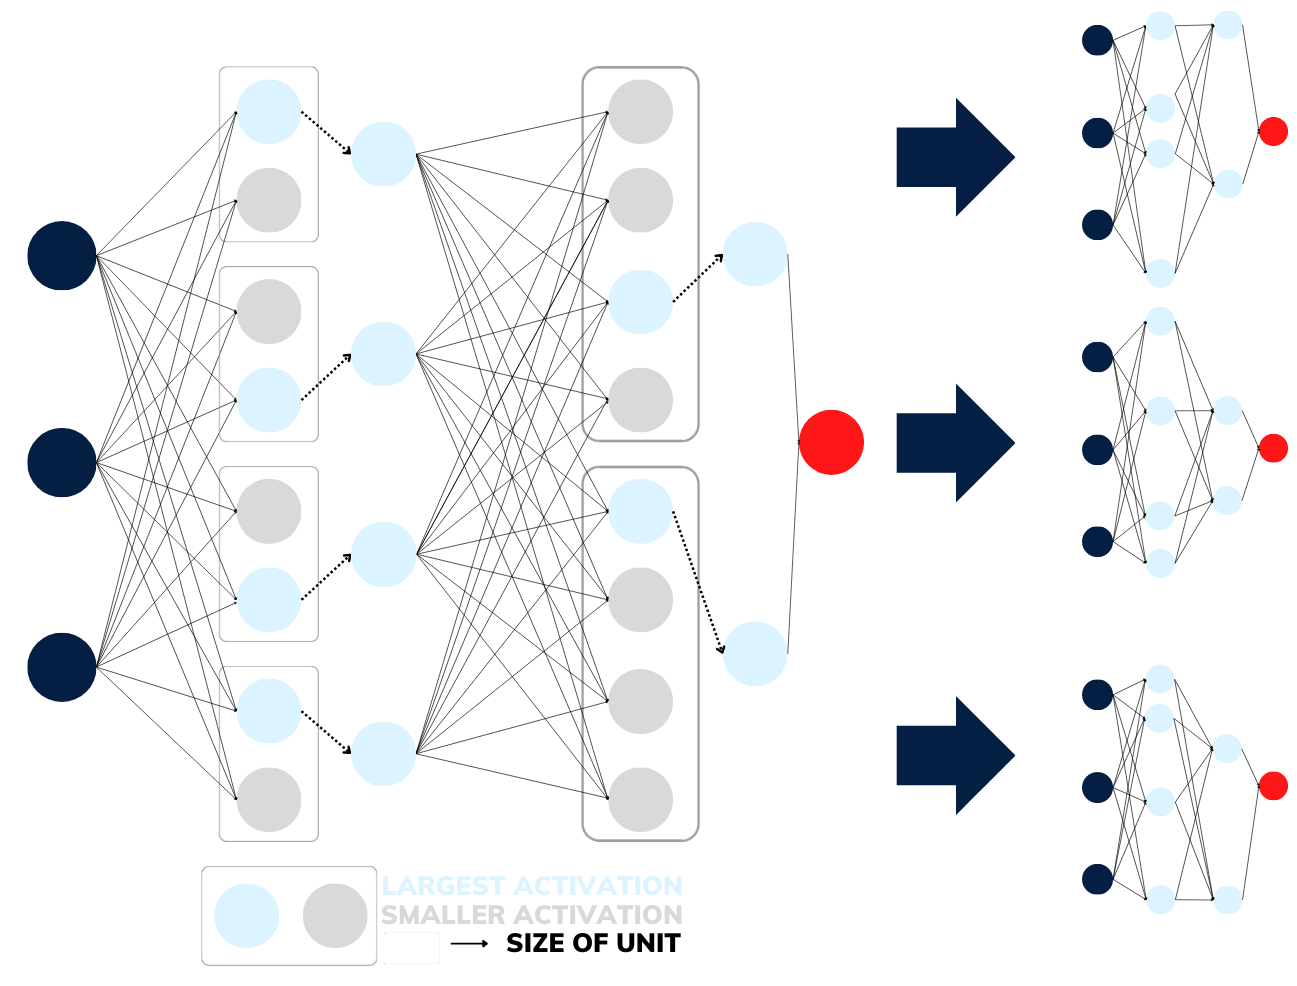
\includegraphics[width=0.7\textwidth]{Figures/Illustrations/Max_out.png}
    \caption[An illustration of a Neural network with two hidden layers using the maxout layer.]{An illustration of a Neural network 
    with two hidden layers, each with 8 neurons. The first and second hidden layers have a maxout activation layer with four and two 
    units respectively. The figure also illustrates the resulting ensemble of smaller neural networks as a consequence
    of the maxout activation layers. }
    \label{fig:Max_out}
\end{figure}
In figure \ref{fig:Max_out} I have illustrated a maxout network. The figure shows a \ac{NN} with two hidden layers
with eight nodes each. In the first hidden layer the maxout layer creates four units, each containing two nodes, and in the 
second layer the maxout creates two units with four nodes each. The resulting output from the first layer is the 
four nodes with the highest activation in their respected unit, likewise the second layer's output is two nodes.
To the right of the network in figure \ref{fig:Max_out}, I have illustrated how the different configuration of 
paths through the network creates an ensemble of networks with their own architecture. Note in the figure how, as described in the 
previous paragraph, each node possesses its own connections to the previous layer, while sharing the connections with the 
rest of the unit, to the next. In figure \ref{fig:NetEnsembleComp} I have drawn a separate illustration to show how 
this differs from both channel-out and \ac{SCO} in this regard. Figure \ref{fig:NetEnsembleComp} illustrates how 
all three layers redimensionalize the network, how channelout and \ac{SCO} differ from maxout in regard to the relationship 
between units and parameters and finally how channel-out differs from \ac{SCO} in choice of units\footnote{In figure 
\ref{fig:NetEnsembleComp} this is highlighted by the different colors surrounding the nodes in \ac{SCO}, where each color 
represents a unit.}
\begin{figure}
    \centering
    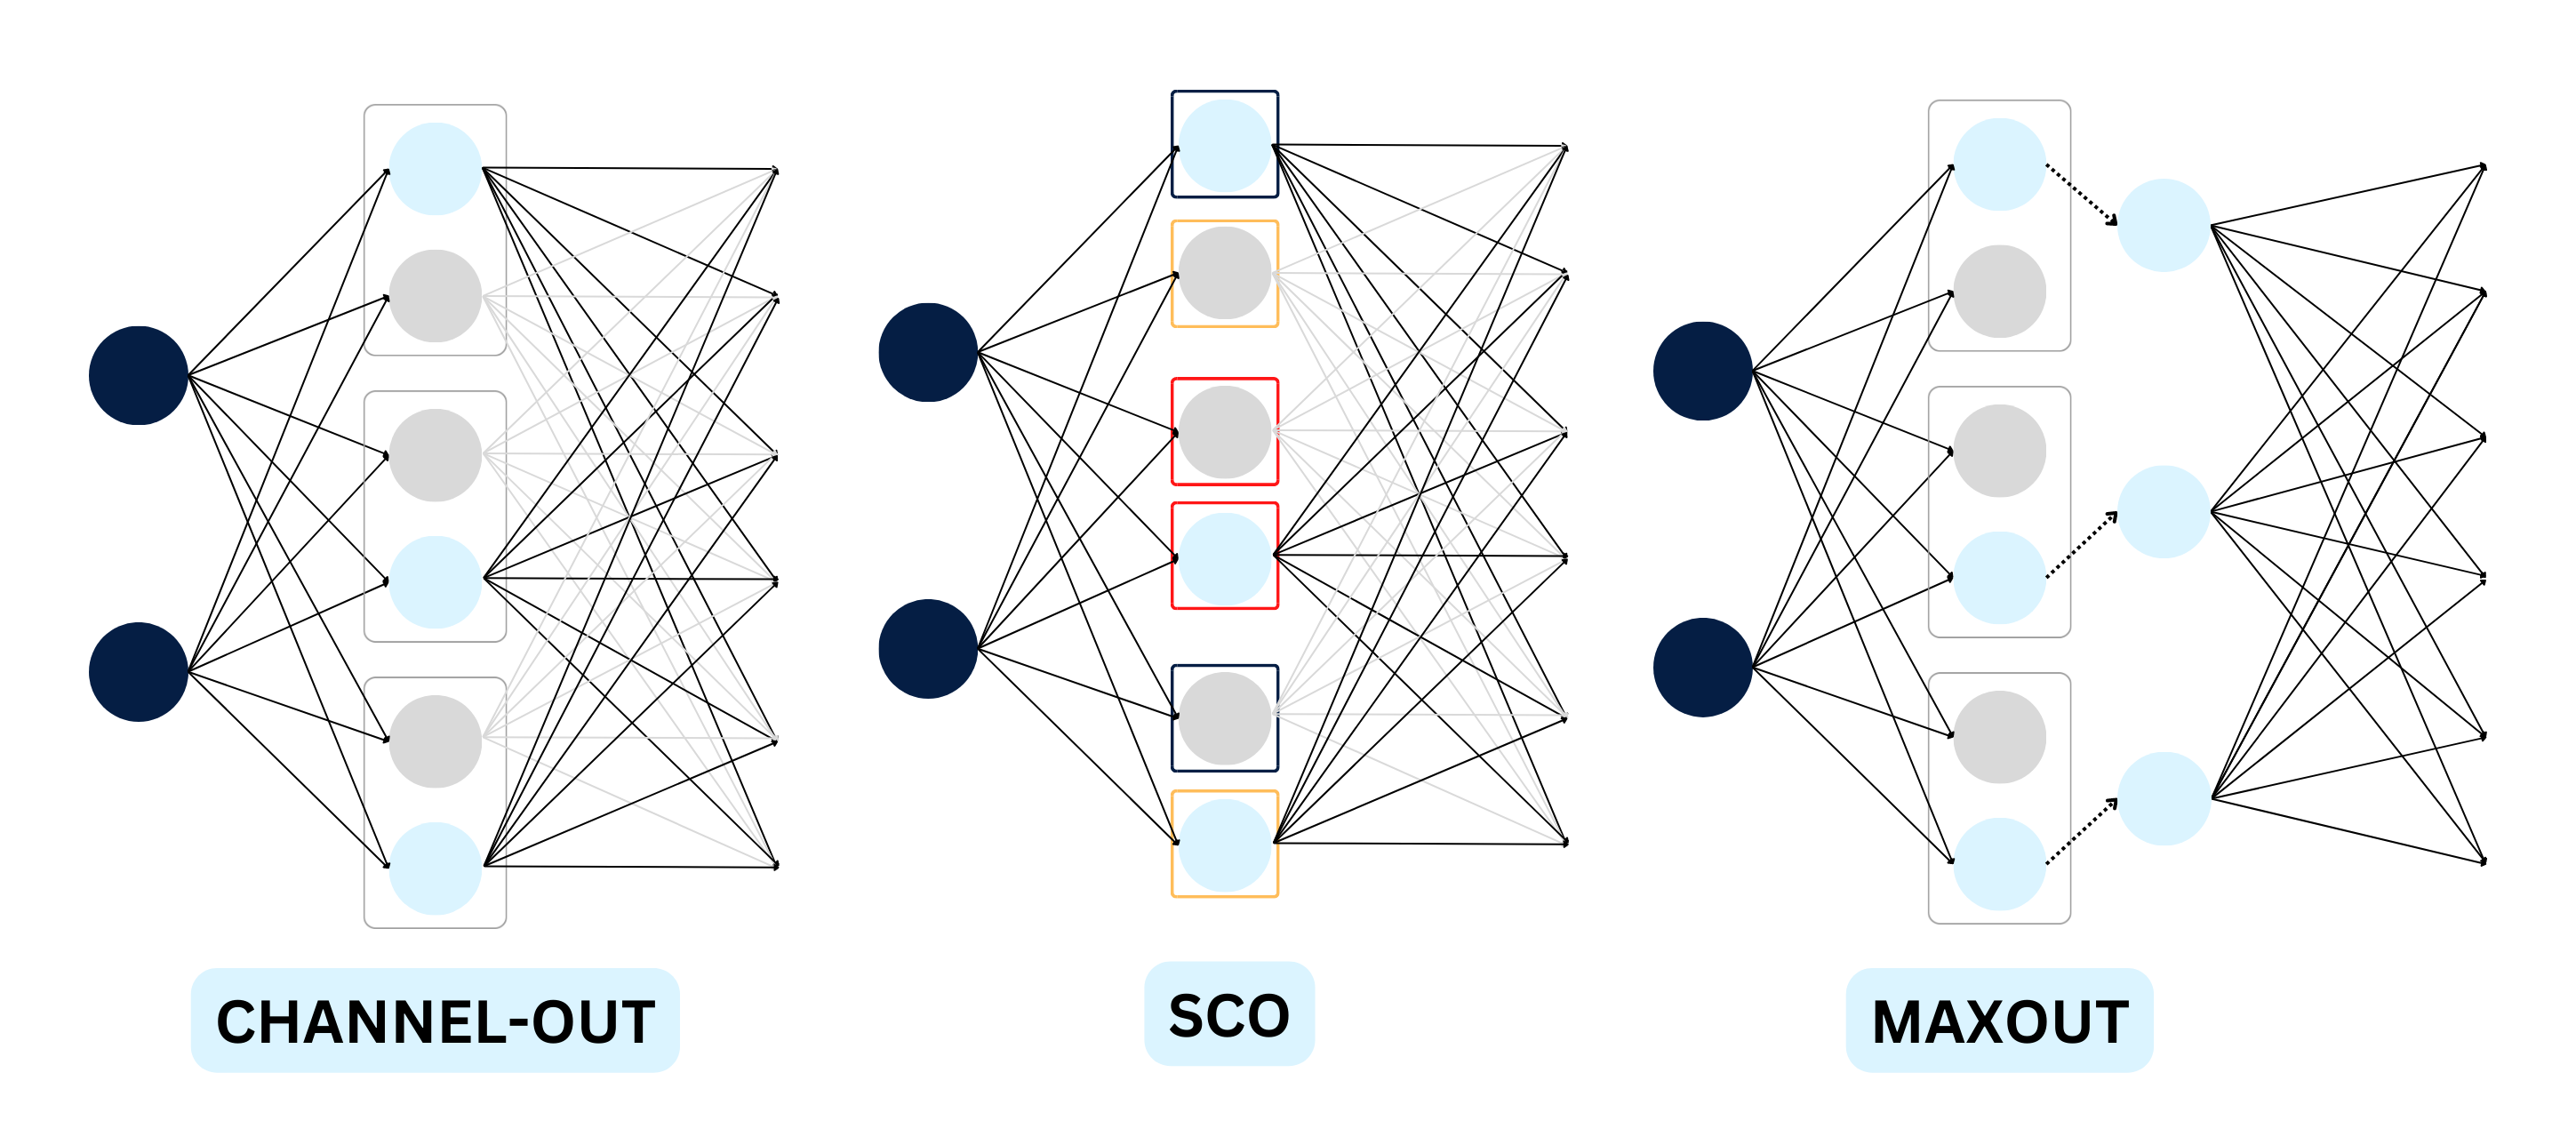
\includegraphics[width=0.8\textwidth]{Figures/Illustrations/EnsembleComp.png}
    \caption[An illustration of three different layers, channelout, \acs{SCO} and maxout.]{An illustration of three different layers, channelout, 
    \ac{SCO} and maxout. The figure shows how each layer redimensionalize the network and how channelout and \ac{SCO} differ from maxout in regard 
    to the relationship between units and parameters. The gray lines and nodes represent dropped nodes, whereas the blue nodes and dark lines represent
    the nodes which are allowed to contribute. In the case of \ac{SCO} the different colors surrounding the nodes represents different units, which 
    visualizes how any set of nodes could define a unit.}
    \label{fig:NetEnsembleComp}
\end{figure}
\subsection{Parametrized Neural Network}\label{subsec:PNN}
In this thesis I will be studying \ac{BSM}-simulations produced with a diversity in choice of free parameters. This
means that the signal is itself diverse. The free parameters studied in this thesis are the mass of 
new particles. The mass of a hypothetical particle in a given \ac{BSM} theory can greatly alter the feature space
spanned by processes including said particle. This means that a single \ac{ML}-model could potentially struggle to tune 
according to multiple signal samples that differ only in the mass of the hypothetical particle. The obvious solution to 
this problem is simply to implement one model per mass combination, or choice of mass, and simply reusing the background. 
Although this approach is very popular, I have decided not to use it for (mainly) three reasons:
\begin{itemize}
    \item This approach has been carefully studied for many years, and leaves little room to further exploration. 
    \item Some signals overlap in the feature space. This means that by neglecting signals with relative 
          similar mass, you could be neglecting statistics which could help tune to your original signal. 
    \item By including two signals with relatively similar masses in the training, some\footnote{See the paper by Baldi et al. \cite{PNN}.} 
          suggest that the model would be able to interpolate between the masses and cover a larger search area.
\end{itemize}
When the data set, $X$, is dependent on a set of free parameters, $\theta = [\theta_0,\theta_1,\theta_2,...,\theta_N]$,
we can write $X(\theta)$. For a single neural network trained on a set of parameters, we define the model as 
$\mathcal{F}(X(\theta))$. In the case where we build one model for each choice of parameter, we get a set of models
defined as $\{ \mathcal{F}_a(X(\theta_a))$, $\mathcal{F}_b(X(\theta_b))$, ...,$\mathcal{F}_c(X(\theta_c))\}$, where
a, b and c are indices which correspond to individual choices of parameters respectively. 
\\
In the paper by Baldi et al. \cite{PNN}, they propose a separate solution to the problem than the one proposed above, the \acf{PNN}. 
By simply including the parameters as additional features, we can write $\mathcal{F}(X, \theta)$. In doing so, 
we can utilize all the statistics at the same time, while also aiding the $\ac{NN}$ in its effort to recognize all individual 
trends for all signals. The difference in approach between parameter specific networks and the \ac{PNN} are highlighted in figure \ref{fig:PNN}.
In practice, it is aiding the \ac{NN} by adding a shift to the total output from the initial layer according to the discrete distribution of the 
parameters. The hope is that each discrete shift will motivate a separate individualistic tuning for each choice of parameter. 
\begin{figure}
    \centering
    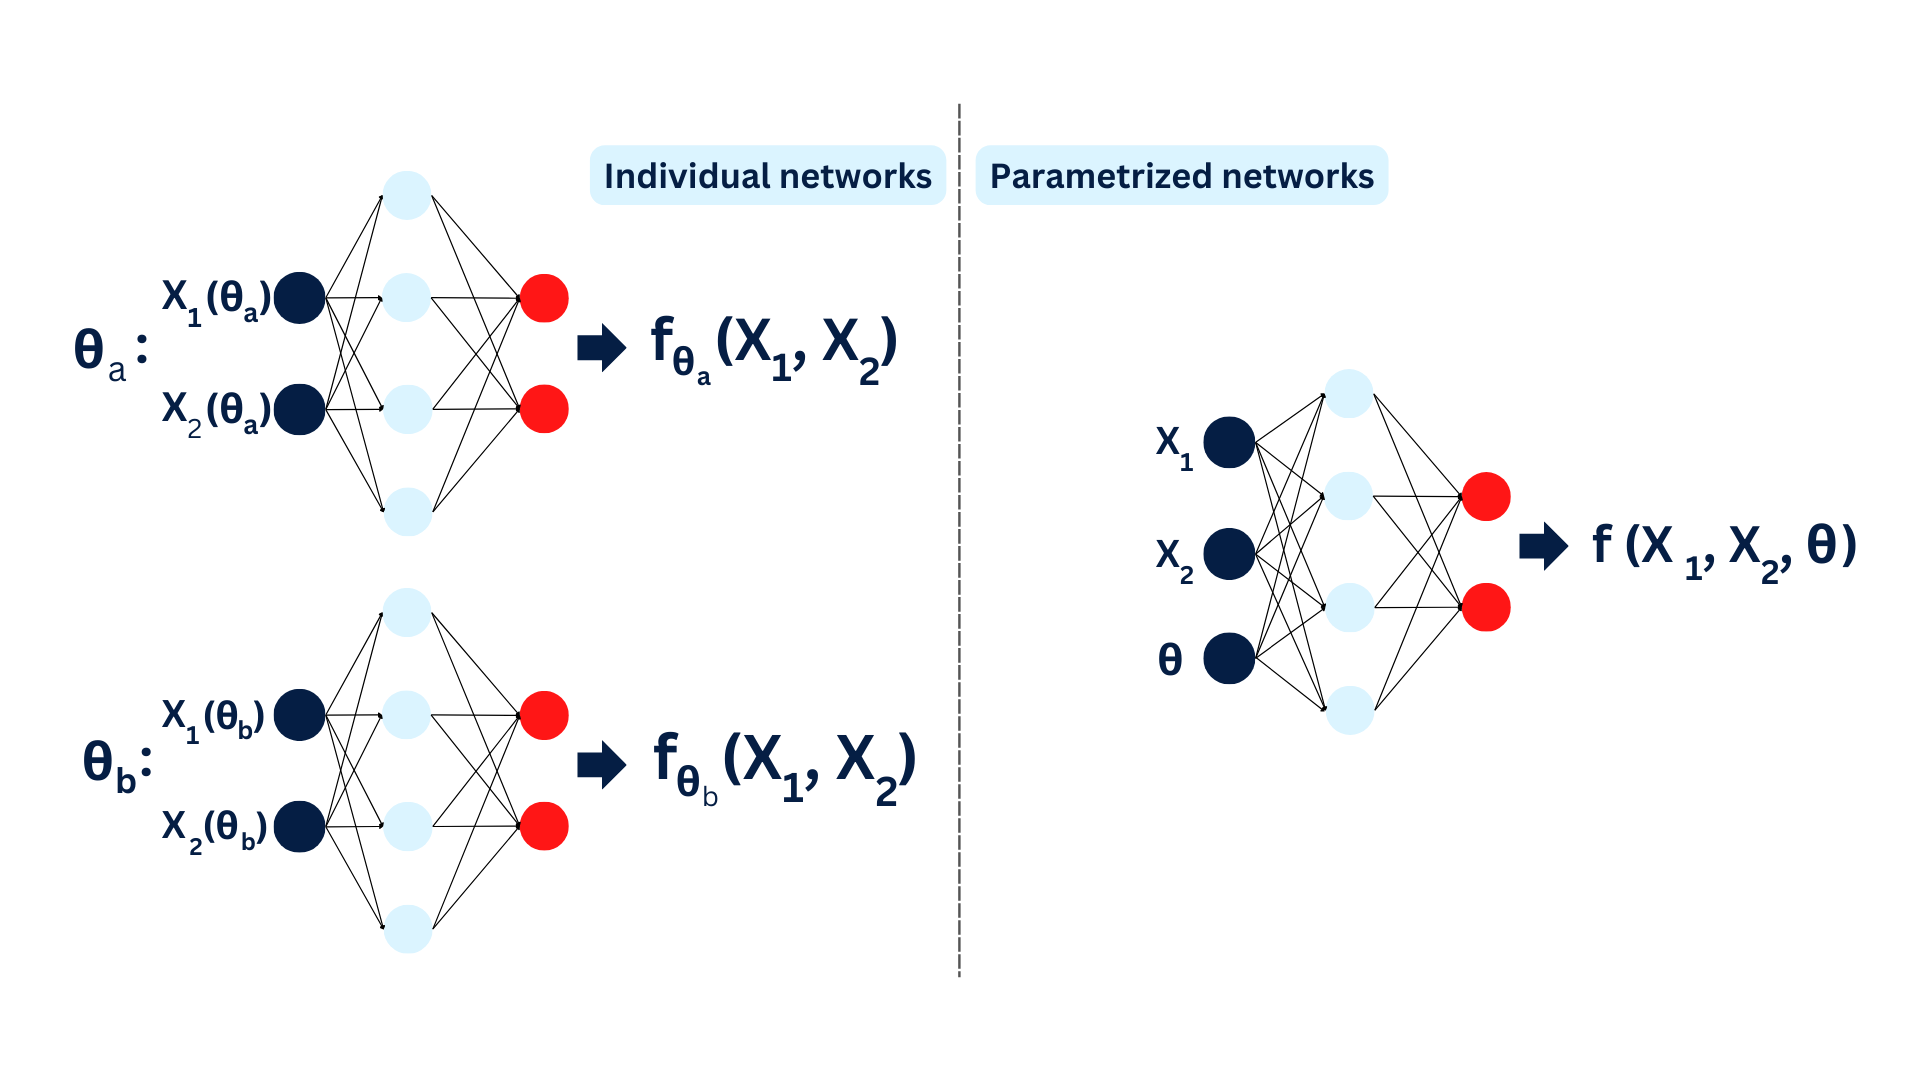
\includegraphics[width=0.8\textwidth]{Figures/Illustrations/PNN.png}
    \vspace{-.8cm}
    \caption{An illustration of a comparison between the parameter individualistic network 
    approach and the \acs{PNN}.}
    \label{fig:PNN}
\end{figure}
For the \ac{SM} background, adding a parameter representing the mass of a \ac{BSM} particle is meaningless. 
Therefore, the background is randomly assigned values according to the same distribution used in the signal data. 
In doing so, one is essentially assigning each set of signal its own portion of background data. 